\section{Results}
\label{sec:results}
\subsection{Selected populations}
Of the simulated lens systems, 51 per cent (SIS) and 42--50 per cent (elliptical families) yield a resolved, detected image pair for ET, and 1.0--1.2 per cent for the O5-like network (Fig.~\ref{fig:population}). ET pairs have median source redshift $z_s\approx2.7$, median delay of about 54\,d and a median brighter-image magnification $\mu_A\approx2.5$. Because the O5-like network must detect both images, its sample is strongly affected by magnification bias. Its pairs lie at lower redshift ($z_s\approx1.9$), are more strongly magnified (median $\mu_A=4.3$--5.2) and contain quadruple-image systems in 33--39 per cent of the elliptical cases, compared with 5--7 per cent for ET. These fractions agree with earlier forecasts of a large quad fraction among magnification-selected lensed BBHs \citep{li2018statistical,wierda2021beyond}. The brighter GW image is the saddle-point image in 14--20 per cent of ET pairs and 28--37 per cent of O5 pairs, because antenna patterns differ between arrival times.

\begin{figure*}
\centering
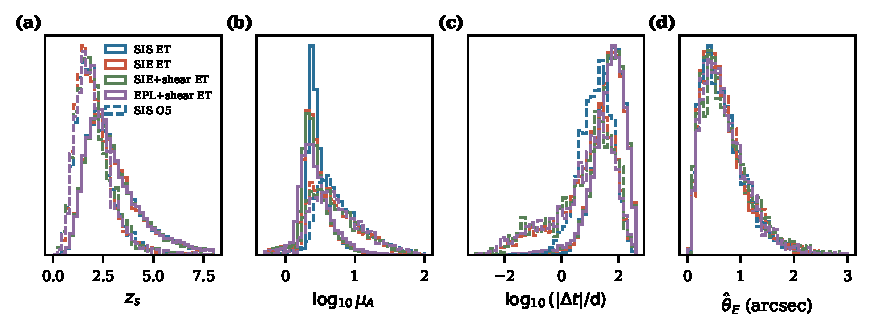
\includegraphics[width=\linewidth]{fig_population.pdf}
\caption{Selected lensed pairs for ET (solid) and the O5-like network (dashed): source redshift, magnification of the brighter GW image, time delay and Einstein-radius proxy, per lens family.}
\label{fig:population}
\end{figure*}

\subsection{Information content of the observables}
\label{sec:information}
Table~\ref{tab:inputs} and Fig.~\ref{fig:inputs} compare the input sets for HistGB estimators trained and tested within each lens family (in-family), and for one NPE trained on all families. Four results stand out.

\emph{Image geometry dominates.} For ET, geometry alone gives median relative errors of 3.2, 7.3, 11.6 and 19.9 per cent for SIS, SIE, SIE+shear and EPL+shear lenses, against 19--32 per cent for the prior-only predictor. Adding the redshifts and velocity dispersion does not help (Geometry+FU), because the image configuration already fixes the dimensionless source position, and $\sigma_v$ with 10 per cent errors constrains the Einstein radius less precisely than the image positions do. The error grows with the number of unobserved lens degrees of freedom: external shear and, above all, the radial slope of the EPL family change the magnification at fixed image configuration.

\emph{The dimensionless GW observables are complementary.} GW data alone give 7.7 per cent for SIS---where the relative magnification fixes $y$ through equation~(\ref{eq:sis})---but 21--26 per cent for the elliptical families. Combined with geometry, the GW relative magnification and arrival order alone (Geometry+GW(ratio)) reduce the SIE+shear error from 11.6 to 10.2 per cent and the EPL+shear error from 19.9 to 18.8 per cent. These inputs are invariant under the mass-sheet transformation and contain no distance scale; this is the scale-free benchmark of our study.

\emph{The delay and the SNRs add information only through the distance scale.} Adding $\ln|\Delta t|$ and the two SNRs without redshifts (Geometry+GW(rel)) changes the errors by at most 0.7 percentage points. With redshifts, however, adding only the delay to Geometry+GW(ratio)+FU improves the EPL+shear error from 18.7 to 16.7 per cent, whereas adding only the SNRs leaves it at 18.2 per cent; all dimensional inputs together give 16.4 per cent. The neural posterior estimator exploits this much more: with Geometry+GW(rel)+FU it reaches 1.7, 5.9, 9.7 and 13.6 per cent, against 3.4, 7.2, 10.6 and 19.8 per cent with the scale-free Geometry+GW(ratio)+FU inputs. The reason is that $\Delta t=(1+z_l)D_{\Delta t}\Delta\phi/c$, so the delay, the redshifts and the simulated cosmology fix the Fermat-potential difference, which constrains the radial slope that geometry leaves free. This information is real only if the distance scale is known. Table~\ref{tab:response} quantifies the dependence. Rescaling all distances by $1/h$ at fixed redshift, as a Hubble constant $h$ times the simulated one would, shifts the Geometry+GW(rel)+FU NPE estimate by ${\rm d}\ln\hat\mu/{\rm d}\ln h=0.69$ for ET and 0.44 for O5, so a 10 per cent error in the assumed $H_0$ biases the magnification by 7 (4) per cent. Scale-free estimators are unaffected to numerical precision. The same NPE estimates respond to an external mass sheet with ${\rm d}\ln\hat\mu/{\rm d}\ln\lambda=-0.69$, whereas the truth scales as $-2$: they partly absorb $\kappa_{\rm ext}$ by misattributing the shorter delay to a steeper lens, but cannot correct for it. HistGB estimates respond less to these transformations (${\rm d}\ln\hat\mu/{\rm d}\ln h=0.13$ for ET), because decision trees predict constant values outside the range of their training data; they are therefore less sensitive to the assumed cosmology but gain correspondingly less from it.

\emph{Known redshift plus cosmology is not competitive on its own.} Inverting the apparent distance with the source redshift gives 41 per cent errors for all families, because the inclination--distance degeneracy calibrated on real events (Section~\ref{sec:realdata}) limits the apparent distance of a single image to $\sigma_{\ln D}\gtrsim0.22$, i.e. $\gtrsim45$ per cent in magnification. Section~\ref{sec:pe} shows that full parameter estimation of both images reduces this floor. Closed-form SIS inversions perform well only when the SIS model is correct and degrade to 21--43 per cent for the elliptical families. A flexible estimator trained on a realistic lens prior is therefore essential.

For the O5-like network all errors are larger (Table~\ref{tab:inputs}b): 10.7, 16.2, 21.9 and 27.9 per cent with geometry and 10.8, 14.8, 18.8 and 25.5 per cent with Geometry+GW(ratio). This is because magnification bias selects highly magnified, near-caustic configurations. The errors stop decreasing above about $10^4$ training events (Fig.~\ref{fig:learning} in Appendix~\ref{app:extra}), so the ET results are not limited by sample size; the smaller O5 samples (1500--3000 per family) cost about 1--2 percentage points.

\begin{table*}
\centering\papertablestyle
\caption{Median relative error $|\hat\mu_A-\mu_A|/\mu_A$ (per cent) of the magnification of image $A$ (larger measured SNR). Parentheses: empirical coverage of the conformal 90 per cent intervals (binomial standard error per division 0.003 for ET and 0.01--0.02 for O5). Top: closed-form estimators. Middle: HistGB trained and tested on the same family, means over five random divisions into training, calibration and test events (standard deviation between divisions below 0.3 percentage points for ET and 1.5 for O5). Bottom: one NPE trained on all four families, with intervals calibrated per true family, which is not possible for real lenses (see Table~\ref{tab:calibration}). Prior only: percentiles of the simulated population, ignoring the event data. FU: follow-up redshifts and velocity dispersion. $^\dagger$Scale-free input sets (Table~\ref{tab:inputsets}).}
\label{tab:inputs}
\textbf{(a) ET}\par\smallskip
\begin{tabular*}{\linewidth}{@{\extracolsep{\fill}}lcccc@{}}
\toprule
Input set & SIS & SIE & SIE+shear & EPL+shear \\
\midrule
SIS analytic (geometry) & 3.3 & 21.0 & 23.8 & 32.9 \\
SIS analytic (GW relative) & 8.7 & 33.0 & 36.5 & 42.5 \\
Known $z_s$ + cosmology & 40.8 & 41.6 & 41.4 & 41.3 \\
\midrule
Prior only$^\dagger$ & 18.7 (0.90) & 24.3 (0.90) & 25.0 (0.90) & 31.6 (0.90) \\
GW & 7.7 (0.90) & 21.4 (0.90) & 21.9 (0.90) & 25.8 (0.90) \\
GW+$z$ & 6.7 (0.90) & 16.9 (0.90) & 17.3 (0.90) & 19.4 (0.90) \\
Geometry$^\dagger$ & 3.2 (0.90) & 7.3 (0.90) & 11.6 (0.90) & 19.9 (0.90) \\
Geometry+FU$^\dagger$ & 3.2 (0.90) & 7.3 (0.90) & 11.6 (0.90) & 19.8 (0.90) \\
Geometry+GW(ratio)$^\dagger$ & 3.0 (0.90) & 6.9 (0.90) & 10.2 (0.90) & 18.8 (0.90) \\
Geometry+GW(ratio)+FU$^\dagger$ & 3.0 (0.90) & 7.0 (0.90) & 10.2 (0.90) & 18.7 (0.90) \\
Geometry+GW(rel) & 2.9 (0.90) & 6.9 (0.90) & 9.9 (0.90) & 18.1 (0.90) \\
Geometry+GW(rel)+FU & 2.7 (0.90) & 6.9 (0.90) & 9.9 (0.90) & 16.4 (0.90) \\
Full & 2.7 (0.90) & 6.9 (0.90) & 10.0 (0.90) & 15.6 (0.90) \\
\midrule
NPE: GW & 9.7 (0.90) & 22.4 (0.90) & 23.9 (0.90) & 27.5 (0.89) \\
NPE: Geometry$^\dagger$ & 3.4 (0.90) & 7.3 (0.90) & 11.9 (0.89) & 20.9 (0.90) \\
NPE: Geometry+GW(ratio)$^\dagger$ & 3.3 (0.90) & 6.8 (0.90) & 10.6 (0.89) & 19.6 (0.89) \\
NPE: Geometry+GW(ratio)+FU$^\dagger$ & 3.4 (0.90) & 7.2 (0.90) & 10.6 (0.89) & 19.8 (0.90) \\
NPE: Geometry+GW(rel) & 3.3 (0.90) & 6.7 (0.90) & 10.2 (0.89) & 18.8 (0.89) \\
NPE: Geometry+GW(rel)+FU & 1.7 (0.89) & 5.9 (0.90) & 9.7 (0.90) & 13.6 (0.90) \\
NPE: Full & 1.8 (0.90) & 6.0 (0.90) & 9.8 (0.90) & 13.8 (0.90) \\
\bottomrule
\end{tabular*}
\par\bigskip\textbf{(b) O5-like network}\par\smallskip
\begin{tabular*}{\linewidth}{@{\extracolsep{\fill}}lcccc@{}}
\toprule
Input set & SIS & SIE & SIE+shear & EPL+shear \\
\midrule
SIS analytic (geometry) & 9.7 & 45.3 & 54.5 & 58.0 \\
SIS analytic (GW relative) & 34.2 & 59.6 & 63.7 & 63.2 \\
Known $z_s$ + cosmology & 46.0 & 49.2 & 53.1 & 50.4 \\
\midrule
Prior only$^\dagger$ & 49.7 (0.91) & 53.5 (0.89) & 52.9 (0.91) & 55.8 (0.90) \\
GW & 29.5 (0.91) & 35.3 (0.90) & 35.4 (0.90) & 34.8 (0.88) \\
GW+$z$ & 19.0 (0.92) & 26.5 (0.89) & 26.8 (0.90) & 29.2 (0.90) \\
Geometry$^\dagger$ & 10.7 (0.90) & 16.2 (0.90) & 21.9 (0.91) & 27.9 (0.88) \\
Geometry+FU$^\dagger$ & 10.7 (0.90) & 16.3 (0.89) & 23.4 (0.91) & 27.9 (0.91) \\
Geometry+GW(ratio)$^\dagger$ & 10.8 (0.90) & 14.8 (0.89) & 18.8 (0.90) & 25.5 (0.90) \\
Geometry+GW(ratio)+FU$^\dagger$ & 10.5 (0.90) & 15.0 (0.89) & 19.4 (0.90) & 25.7 (0.90) \\
Geometry+GW(rel) & 9.9 (0.90) & 15.4 (0.90) & 17.9 (0.90) & 24.8 (0.89) \\
Geometry+GW(rel)+FU & 8.8 (0.91) & 14.7 (0.90) & 18.3 (0.89) & 24.6 (0.90) \\
Full & 8.8 (0.91) & 15.7 (0.90) & 17.7 (0.90) & 24.2 (0.89) \\
\midrule
NPE: GW & 29.3 (0.91) & 36.3 (0.88) & 39.7 (0.89) & 36.6 (0.89) \\
NPE: Geometry$^\dagger$ & 11.3 (0.89) & 14.3 (0.92) & 22.6 (0.90) & 24.8 (0.90) \\
NPE: Geometry+GW(ratio)$^\dagger$ & 10.4 (0.89) & 12.4 (0.90) & 18.0 (0.90) & 27.2 (0.91) \\
NPE: Geometry+GW(ratio)+FU$^\dagger$ & 10.6 (0.89) & 13.1 (0.89) & 17.3 (0.89) & 27.6 (0.91) \\
NPE: Geometry+GW(rel) & 11.4 (0.91) & 12.3 (0.91) & 20.1 (0.90) & 26.2 (0.92) \\
NPE: Geometry+GW(rel)+FU & 7.2 (0.90) & 10.7 (0.91) & 15.0 (0.92) & 21.3 (0.94) \\
NPE: Full & 7.3 (0.91) & 11.1 (0.89) & 15.4 (0.92) & 19.4 (0.93) \\
\bottomrule
\end{tabular*}
\end{table*}

\begin{table*}
\centering\papertablestyle
\caption{Response of the predicted magnification to an external mass sheet ($\lambda=1-\kappa_{\rm ext}$; the truth scales as ${\rm d}\ln\mu/{\rm d}\ln\lambda=-2$) and to a distance scale $1/h$ at fixed redshift (the truth is unchanged). Slopes from $\pm10$ per cent transformations of the fixed test systems. GW(ratio+clock) and GW(ratio+SNR) add only $\ln|\Delta t|$ or only the SNRs to GW(ratio).}
\label{tab:response}
\begin{tabular*}{\linewidth}{@{\extracolsep{\fill}}llcccc@{}}
\toprule
 & & \multicolumn{2}{c}{${\rm d}\ln\hat\mu/{\rm d}\ln\lambda$} & \multicolumn{2}{c}{${\rm d}\ln\hat\mu/{\rm d}\ln h$} \\
Scen. & Input set & HistGB & NPE & HistGB & NPE \\
\midrule
ET & Geometry+GW(ratio)+FU & +0.00 & +0.00 & +0.00 & +0.00 \\
ET & Geometry+GW(rel) & -0.03 & -0.04 & +0.03 & +0.04 \\
ET & Geometry+GW(ratio+clock)+FU & -0.10 & -- & +0.10 & -- \\
ET & Geometry+GW(ratio+SNR)+FU & -0.03 & -- & +0.03 & -- \\
ET & Geometry+GW(rel)+FU & -0.13 & -0.69 & +0.13 & +0.69 \\
ET & Full & -0.21 & -0.71 & +0.21 & +0.71 \\
O5 & Geometry+GW(ratio)+FU & +0.00 & -0.00 & +0.00 & -0.00 \\
O5 & Geometry+GW(rel) & -0.08 & -0.15 & +0.09 & +0.14 \\
O5 & Geometry+GW(ratio+clock)+FU & -0.03 & -- & +0.03 & -- \\
O5 & Geometry+GW(ratio+SNR)+FU & -0.08 & -- & +0.08 & -- \\
O5 & Geometry+GW(rel)+FU & -0.14 & -0.43 & +0.13 & +0.44 \\
O5 & Full & -0.30 & -0.56 & +0.30 & +0.56 \\
\bottomrule
\end{tabular*}
\end{table*}

\begin{figure*}
\centering
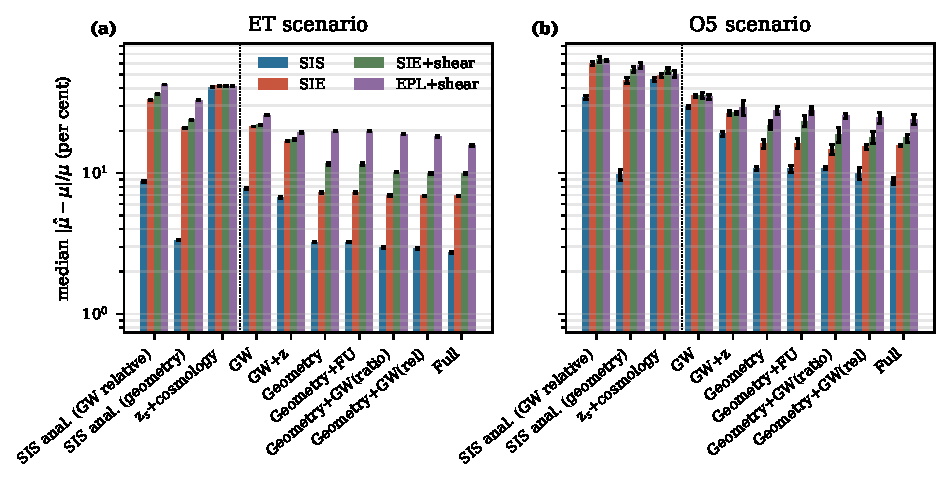
\includegraphics[width=\linewidth]{fig_inputs.pdf}
\caption{Median relative magnification error by input set and lens family (in-family training; error bars: standard deviation over five random divisions). Left of the dotted line: closed-form estimators.}
\label{fig:inputs}
\end{figure*}

\subsection{Near-caustic configurations}
Errors grow rapidly with magnification (Fig.~\ref{fig:tail}). With the scale-free Geometry+GW(ratio) inputs for ET, the median relative error rises from 2--13 per cent at $2<\mu_A<3$ to 10--34 per cent at $5<\mu_A<10$ and 44--57 per cent at $\mu_A>20$. This is the behaviour expected from $\delta\ln\mu=-\operatorname{tr}(A^{-1}\delta A)$: near a fold the same astrometric and model uncertainty produces a magnification error proportional to $\mu$. The rise at $\mu_A<2$ reflects demagnified saddle images that are brighter in SNR only because of the antenna pattern. Intervals calibrated over the whole population contain the truth too rarely in the high-magnification tail (coverage 0.65--0.80 at $10<\mu_A\le20$ and 0.44--0.57 above 20), even though they cover 90 per cent of events overall (Section~\ref{sec:calibration}). Neural posterior estimation with the same scale-free inputs reduces the tail errors only moderately, to 30--46 per cent at $\mu_A>20$. With the delay and redshifts (Geometry+GW(rel)+FU) the tail errors fall to 6--21 per cent, because near a caustic the delay $\Delta t\propto y\,\theta_E^2D_{\Delta t}$ fixes the dimensionless source position once $D_{\Delta t}$ is known. This gain therefore relies on the assumed cosmology and on $\kappa_{\rm ext}=0$.

\begin{figure*}
\centering
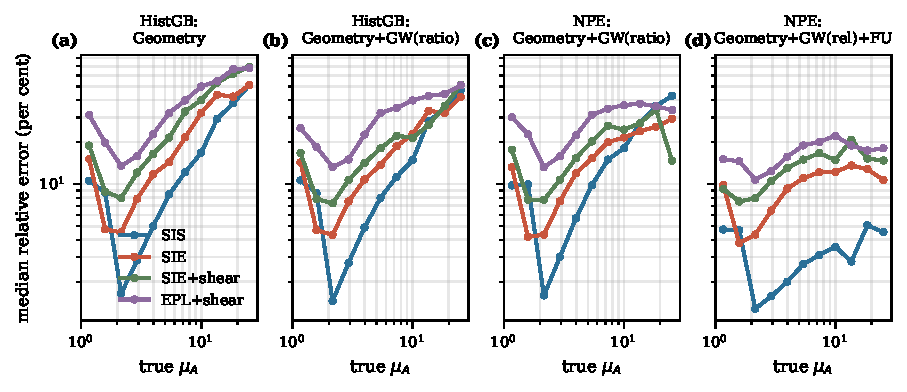
\includegraphics[width=\linewidth]{fig_tail.pdf}
\caption{Median relative error versus true magnification for ET. (a), (b) In-family HistGB models with Geometry and the scale-free Geometry+GW(ratio) inputs (test events of one random division); (c), (d) NPE trained on all families with the scale-free Geometry+GW(ratio) and the scale-dependent Geometry+GW(rel)+FU inputs.}
\label{fig:tail}
\end{figure*}

\subsection{Calibration of the uncertainties}
\label{sec:calibration}
Within a single lens family, CQR intervals achieve the nominal coverage for every input set and both scenarios (0.88--0.92; Table~\ref{tab:inputs}). A single model trained on all four families is almost as accurate as the in-family models (3.4, 7.1, 11.0 and 20.0 per cent with Geometry+GW(ratio) for ET), but a single conformal correction for all families is wrong for each of them. It over-covers SIS and SIE (0.95--0.97) and under-covers EPL+shear (0.75), because the families have different error distributions (Table~\ref{tab:calibration}, Fig.~\ref{fig:coverage}a). Calibrating separately per true family restores 0.90 coverage in every family, but the true family of a real lens is not known. Calibration groups defined by observables do not reproduce it: grouping by the number of images or by the predicted magnification leaves the EPL+shear coverage at 0.75--0.76, because these observables hardly distinguish the families. What does work without a family label is to calibrate on the most flexible family alone. Conformal correction computed on the EPL+shear calibration events gives coverage of at least 0.90 in every family, at the price of 40 per cent wider intervals and over-coverage (0.98--0.99) for the simpler families. The O5 results are similar (Table~\ref{tab:calibration}b).

The conformal guarantee holds on average over the population, or within any group of events defined by \emph{observed} quantities, but not within groups defined by the unobserved true magnification. We therefore also calibrated in-family models in five bins of the \emph{predicted} magnification (Fig.~\ref{fig:coverage}b). By construction this restores 90 per cent coverage in every predicted-magnification bin, but coverage in bins of the true magnification hardly changes: averaged over families it is 0.84, 0.75 and 0.54 for true $\mu_A$ in $(5,10]$, $(10,20]$ and above 20 for ET, against 0.82, 0.73 and 0.51 with a single calibration for all magnifications. Truly near-caustic events are under-covered because, given the measurement noise, they are partly indistinguishable from moderately magnified configurations, and the estimators pull them towards typical magnifications. This is a remaining failure of all calibrated estimators in our study, not one that predicted-magnification calibration solves. Interval widths must therefore be interpreted as conditional on the observables, and analyses that select events by high inferred magnification should account for this regression to the mean.

Neural posterior estimation provides full posteriors. Trained once on all four families with the scale-free Geometry+GW(ratio) inputs for ET, the posterior median reaches 3.3, 6.8, 10.6 and 19.6 per cent, comparable to the in-family HistGB models (3.0, 6.9, 10.2 and 18.8 per cent) without access to the family label. Its raw posteriors are calibrated over the whole population but not per family (coverage 0.94, 0.97, 0.92 and 0.76; Fig.~\ref{fig:coverage}c): the network learns an average error distribution, exactly like the global conformal correction. The same calibration choices apply. Per-true-family recalibration restores 0.89--0.90 in every family; observable groups do not; EPL+shear calibration gives 0.89--0.99. Conformal recalibration adjusts the end points of the 90 per cent interval only and does not by itself certify the rest of the posterior density.

\begin{table*}
\centering\papertablestyle
\caption{Coverage of the 90 per cent intervals per lens family for one model trained on all four families with Geometry+GW(ratio) inputs, for different conformal calibrations. ``Width'' is the mean width of $\ln\mu_A$ intervals over all families. The true-family calibration is a diagnostic only, because the family of a real lens is unknown. HistGB: means over three random divisions; binomial standard errors are below 0.006 (ET) and 0.02 (O5).}
\label{tab:calibration}
\textbf{(a) ET}\par\smallskip
\begin{tabular*}{\linewidth}{@{\extracolsep{\fill}}llccccc@{}}
\toprule
Estimator & Calibration & SIS & SIE & SIE+shear & EPL+shear & width \\
\midrule
HistGB & global & 0.95 & 0.97 & 0.91 & 0.75 & 0.67 \\
HistGB & image multiplicity & 0.95 & 0.97 & 0.92 & 0.76 & 0.67 \\
HistGB & predicted $\mu$ & 0.95 & 0.97 & 0.91 & 0.75 & 0.68 \\
HistGB & EPL+shear only & 0.99 & 0.99 & 0.98 & 0.90 & 0.94 \\
HistGB & true family (diagnostic) & 0.90 & 0.90 & 0.90 & 0.90 & 0.68 \\
\midrule
NPE & global & 0.94 & 0.97 & 0.92 & 0.76 & 0.65 \\
NPE & image multiplicity & 0.94 & 0.97 & 0.92 & 0.76 & 0.65 \\
NPE & predicted $\mu$ & 0.94 & 0.97 & 0.92 & 0.76 & 0.65 \\
NPE & EPL+shear only & 0.99 & 0.99 & 0.98 & 0.89 & 0.91 \\
NPE & true family (diagnostic) & 0.90 & 0.90 & 0.89 & 0.89 & 0.66 \\
\bottomrule
\end{tabular*}
\par\bigskip\textbf{(b) O5-like network}\par\smallskip
\begin{tabular*}{\linewidth}{@{\extracolsep{\fill}}llccccc@{}}
\toprule
Estimator & Calibration & SIS & SIE & SIE+shear & EPL+shear & width \\
\midrule
HistGB & global & 0.92 & 0.92 & 0.87 & 0.81 & 1.13 \\
HistGB & image multiplicity & 0.92 & 0.92 & 0.88 & 0.82 & 1.13 \\
HistGB & predicted $\mu$ & 0.92 & 0.91 & 0.88 & 0.81 & 1.15 \\
HistGB & EPL+shear only & 0.95 & 0.96 & 0.95 & 0.90 & 1.38 \\
HistGB & true family (diagnostic) & 0.88 & 0.90 & 0.88 & 0.90 & 1.11 \\
\midrule
NPE & global & 0.94 & 0.93 & 0.91 & 0.80 & 1.01 \\
NPE & image multiplicity & 0.92 & 0.94 & 0.92 & 0.82 & 1.02 \\
NPE & predicted $\mu$ & 0.94 & 0.94 & 0.91 & 0.80 & 1.02 \\
NPE & EPL+shear only & 0.99 & 0.98 & 0.96 & 0.91 & 1.43 \\
NPE & true family (diagnostic) & 0.89 & 0.90 & 0.90 & 0.91 & 0.98 \\
\bottomrule
\end{tabular*}
\end{table*}

\begin{figure*}
\centering
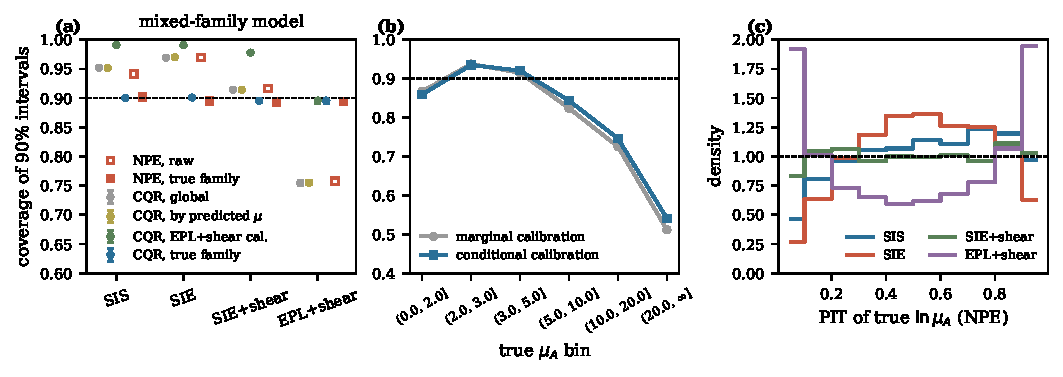
\includegraphics[width=\linewidth]{fig_coverage.pdf}
\caption{Calibration of the 90 per cent intervals for ET (Geometry+GW(ratio) inputs). (a) Coverage per family for a HistGB model trained on all families with global, predicted-magnification, EPL+shear-only and true-family conformal calibration (error bars: scatter between random divisions), and for neural posterior estimation (raw and recalibrated per true family). (b) Coverage in bins of true magnification for a single calibration (``marginal'') and for calibration within bins of predicted magnification (``conditional''); in-family models, mean over families and three random divisions. (c) Histograms of the PIT (posterior probability below the true value) for the NPE; a flat histogram indicates calibrated posteriors.}
\label{fig:coverage}
\end{figure*}

\subsection{Wrong lens-model assumptions}
\label{sec:transfer}
Fig.~\ref{fig:transfer} shows models trained on one family and applied to another. Training on SIS lenses---the default assumption of many lensed-GW forecasts---is the worst choice. Applied to elliptical lenses it gives 21--31 per cent errors with 90 per cent intervals covering only 20--27 per cent of the true values: the SIS prior is confidently wrong. Conversely, the most flexible EPL+shear prior transfers to the simpler families at a moderate accuracy cost (9.4--13.0 per cent instead of 3.0--10.3 per cent in-family) and conservative coverage (0.96--0.98). The SIE and SIE+shear priors transfer well to each other and to SIS, but under-cover EPL+shear lenses (0.48 and 0.61). When SIS, SIE or SIE+shear lenses are omitted from the training set of a model trained on several families, the intervals still cover 91--97 per cent of their true values, at a moderate accuracy cost (for SIS, 3.4 rises to 6.6 per cent), whereas omitting EPL+shear lenses yields 22 per cent errors and coverage 0.55. The radial density slope is thus the dominant lens-model systematic: training sets must include slope variations comparable to those of real lenses, and calibration should use the broadest plausible lens population. This conservative transfer is established only among our four families; real lenses with structure outside the EPL+shear family can still be misdescribed.

\begin{figure*}
\centering
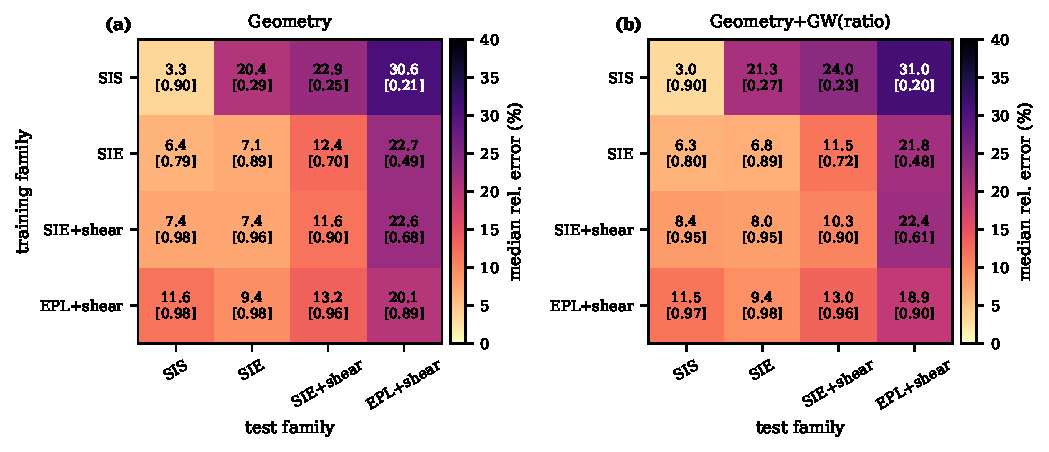
\includegraphics[width=\linewidth]{fig_transfer.pdf}
\caption{Transfer between lens families for ET. Cells give the median relative error (per cent) and, in brackets, the coverage of the 90 per cent intervals, for models trained on the row family and tested on the column family.}
\label{fig:transfer}
\end{figure*}

\subsection{Sky localisation}
The GW relative magnification requires the antenna response of both images, and hence the sky position, polarisation and inclination. With the sky and orientation uncertainties expected for ET alone, the median error of the GW-only SIS estimate is 7.7 per cent; with the sky position known (for example from the identified host galaxy) it falls to 3.9 per cent. Combined with geometry, known sky improves the Geometry+GW(ratio) errors from 10.2 to 8.1 per cent for SIE+shear and from 18.8 to 17.3 per cent for EPL+shear. Host identification therefore also sharpens the GW relative magnification \citep{hannuksela2020localizing,wempe2022lensing}. Because the main benchmark assumes an identified host, its estimated-sky GW errors are conservative; Section~\ref{sec:jointpe} shows that for a single ET detector the known sky also removes occasional wrong solutions of the joint PE.

\subsection{Luminosity distance}
\label{sec:distance}
The magnification correction gives $\hat d_L=\hat D_{{\rm app},A}\,\hat\mu_A^{1/2}$, evaluated event by event, so any correlation between the two estimates is retained. For the scale-free inputs the magnification estimate does not use the apparent distance, so the two errors are independent apart from the shared image SNR. For ET with Geometry+GW(ratio) inputs the magnification contributes a median $|\delta\ln d_L|$ of 1.5, 3.5, 5.1 and 9.5 per cent for SIS, SIE, SIE+shear and EPL+shear. The total median error is 22--24 per cent, almost the same as the 22 per cent obtained with the true magnification (Fig.~\ref{fig:distance}). For O5 the magnification contributes 5--13 per cent, against a total of 27--33 per cent. Under the catalogue-calibrated apparent-distance model, magnification inferred from image geometry is therefore not the limiting factor for the distance of a typical lensed BBH; the exception is a strongly magnified image ($\mu\gtrsim10$). This conclusion depends on the apparent-distance error. The catalogue-calibrated floor $\sigma_{\ln D}\approx0.22$ reflects current detectors, waveform models and the inclination--distance degeneracy; higher harmonics reduce it for third-generation detectors \citep{liu2024harmonics}, and our joint PE gives ET apparent-distance errors about half as large (Section~\ref{sec:jointpe}). With such errors the magnification term is comparable to the GW term for elliptical lenses.

\begin{figure}
\centering
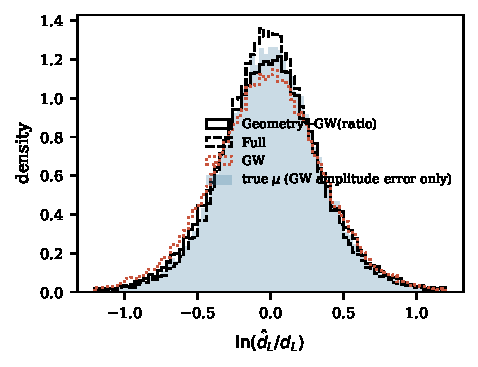
\includegraphics[width=\columnwidth]{fig_distance.pdf}
\caption{Error of the magnification-corrected luminosity distance for ET (all families). The shaded histogram uses the true magnification and shows the GW apparent-distance error alone.}
\label{fig:distance}
\end{figure}
